\documentclass{article}
\usepackage{fullpage}
\usepackage{graphicx}
\usepackage{subfigure}
\usepackage{indentfirst}
\usepackage{float}	  %to make figures not float
\restylefloat{figure} %to make figures not float

\title{CS451 Project 1 \\ Benchmark Evaluations}
\author{Adrian Birylo \\ Daniel Hitchings}

\begin{document}

\bigskip
\maketitle
\bigskip 
\bigskip

\section{Introduction}
This evaluation report aims to report the results of our benchmarking tests, and analyze them for correctness, as well as explain the meaning behind them.  All of our tests were run on a single node on the Jarvis cluster, and so it should be possible to obtain these same (or similar) results.  Each node has an 8-core CPU, 16GB of RAM, and an nVidia GTX 480.

\section{CPU Benchmarks}
This benchmark set out to test the processors capability to conduct both floating point operations and integer operations.  Our method of obtaining these results is explained in the corresponding design document.

\subsection{Data \& Figures}
Below is a table showing the results of our benchmarking tests.  One can see that the number of operations per second reaches a maximum value at 8 threads, and then more or less levels out.  This is understandable, given that the test machine has 8 cores in it's processor.  At this point, the level of hardware concurrency reaches it's maximum.
\begin{figure}[H]
	\centering
	\begin{tabular}{|c|c|c|}
		\hline
		Threads & GIOPS & GFLOPS \\
		\hline
		1 & 2.557749 & 0.987106 \\
		\hline
		2 &	5.116862 &	1.976732 \\
		\hline
		3 &	7.646356 &	2.950336 \\
		\hline
		4 &	10.114046 &	3.854106 \\
		\hline
		5 &	9.029515 &	3.220504 \\
		\hline
		6 &	10.670421 &	3.834759 \\
		\hline
		7 &	11.270062 &	3.834369 \\
		\hline
		8 &	12.760019 &	3.911423 \\
		\hline	
		9 &	10.826525 &	3.641882 \\
		\hline
		10 &	11.530008 &	3.745026 \\
		\hline
		11 &	11.763657 &	3.805008 \\
		\hline
		12 &	12.51453 &	3.910042 \\
		\hline
		13 &	11.810129 &	3.797376 \\
		\hline
		14 &	12.203094 &	3.855521 \\
		\hline
		15 &	12.373366 &	3.879927 \\
		\hline	
		16 &	12.76373 &	3.913256 \\
		\hline
	\end{tabular}
	\caption{CPU Benchmark Results}
\end{figure}

\begin{figure}[H]
	\centering
	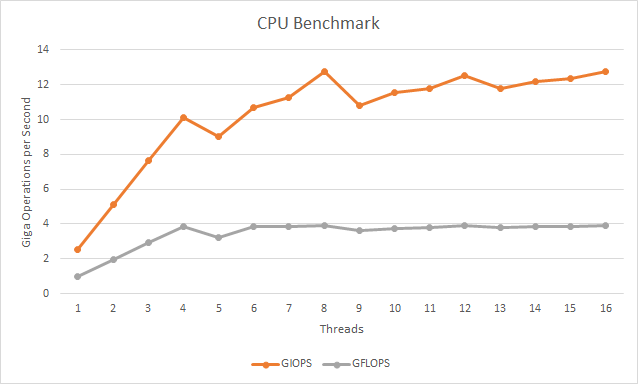
\includegraphics[width=0.7\textwidth]{cpu_bench.png}
	\caption{CPU Operations vs Threads}
\end{figure}
Above is a graph demonstrating the relationship between the number of threads and the operations per second.  It is even clearer here that the operations per sec increase dramatically until hitting 8 threads, and then taper off.

\section{GPU Benchmarks}
This test measures the GPU speed, in terms of operations per second, of both integer and floating point operations.  This test uses the full concurrency of the GPU.

\subsection{Data \& Figures}
\begin{figure}[H]
\center{
\begin{tabular}{|c|c|}
\hline
GIOPS & GFLOPS \\
\hline
1192.321 & 1351.923 \\
\hline
\end{tabular}
\caption{GPU GIOPS and GFLOPS Benchmark}
}
\end{figure}
The number of operations shown above are much higher than the CPU speed, due to the massive concurrency that GPUs allow for.  Even though the processor is most likely running at a lower clock speed, there are over 100 times more cores than a CPU, so the throughput can be much, much larger. \\

\begin{figure}[H]
\center{
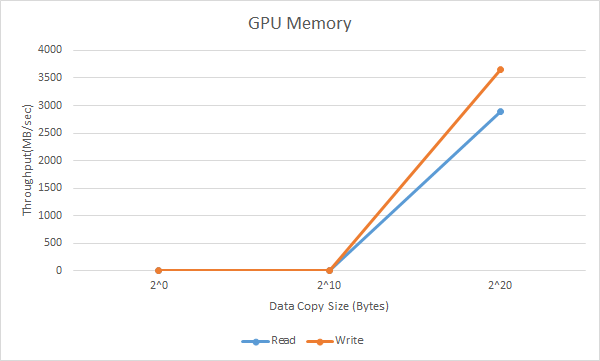
\includegraphics[width=\textwidth]{gpu_mem_bench.png}
\caption{GPU Memory Benchmark}
}
\end{figure}

Above, you can see that using larger block sizes leads to a much higher throughput.  This is for similar reasons as described in the Memory Benchmarks section

\section{Memory Benchmarks}
The memory benchmarking program measures the speed of read/write operations of the RAM in the machine.  This speed is measured in throughput(MB/sec) and latency(ms/byte).  The test was run at varying block sizes (Byte, Kilobyte, and Megabyte) and with a varying number of threads.

\subsection{Data \& Figures}
\begin{figure}[H]
\center{
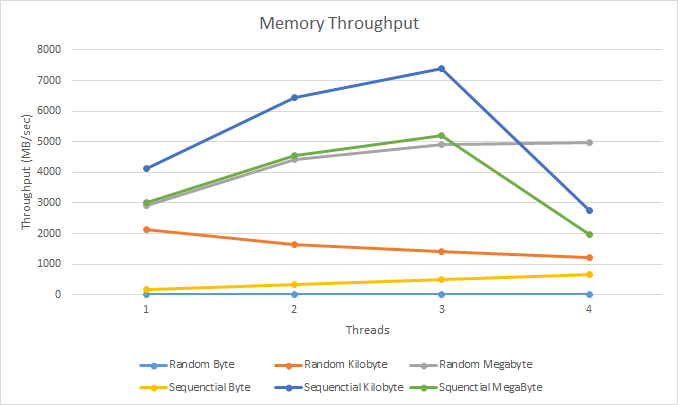
\includegraphics[width=.7\textwidth]{mem_throughput.png}
\caption{Memory Throughput Benchmark}
}
\end{figure}

The throughput maximum happens at 3 threads for most cases.  After this point, there are most likely delays with the memory bus.  The variation in throughput with various block sizes can clearly be seen as well, with the maximum throughput happening with kilobyte block sizes.  A block size of 512KB is common, so we might see even higher speeds if we were to test that block size. \\

\begin{figure}[H]
\center{
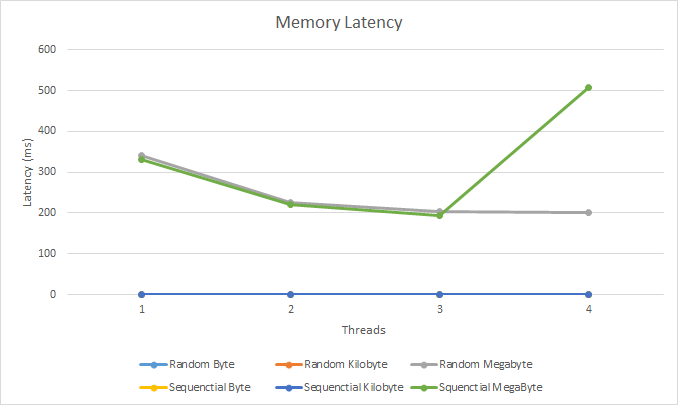
\includegraphics[width=.7\textwidth]{mem_latency.png}
\caption{Memory Latency Benchmark}
}
\end{figure}

The latency is clearly the lowest with byte size block transfers, but since so many more operations have to be done to copy most data structures, the speed here does not lead to a greater overall speed.  This demonstrates how important it is to use more than one metric to determine speed.


\section{Disk Benchmarks}
The disk benchmark measured the hard drive speed, in terms of read operations and write operations, both sequential and random.  This test was run with varying block sizes (Byte, Kilobyte, Megabyte, and Gigabyte) as was as with a varying number of threads.
\subsection{Data \& Figures}
\begin{figure}[H]
\center{
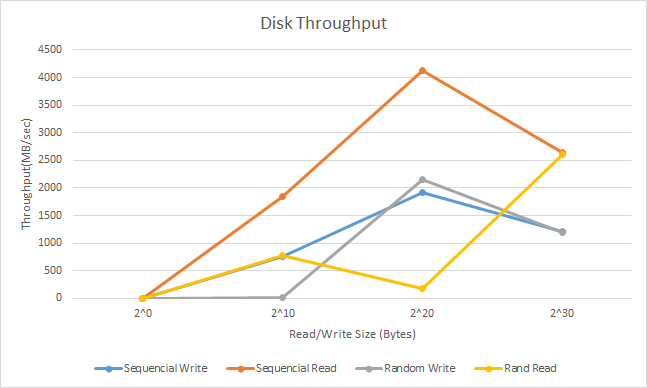
\includegraphics[width=.7\textwidth]{disk_throughput.png}
\caption{Disk Throughput Benchmark}
}

The throughput of reading and writing to a disk reaches a peak at megabyte block sizes.  This is due to the design of the hard drive, and the limiting factor of having physical moving parts.  Having to move the disk for each operation means that small operations have a large amount of overhead.  Similarly, there are a limited number of heads, so a block size larger than that means that they will each have to read/write multiple times.  Finding a balance between those is key.  A commonly used block size is 512KB, so there might actually be a slightly higher peak there, if we were test it.  \\

\end{figure}
\begin{figure}[H]
\center{
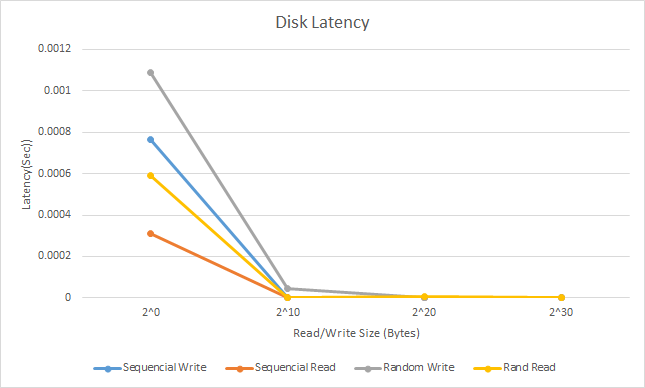
\includegraphics[width=.7\textwidth]{disk_latency.png}
\caption{Disk Latency Benchmark}
}

The latency decreases greatly once dealing with block sizes greater than a single byte.  This again has to do with the physical limitations of having moving parts.  The more the drive needs to move them, the longer a delay there will be.
\end{figure}

\pagebreak
\section{Network Benchmarks}
This benchmark tests the speed of the loopback interface using the UDP protocol.  This test is run using varying buffer sizes (1B, 1KB, and 64KB) and at different levels of concurrency (1 thread and 2 threads).  The results are shown in both throughput(MB/sec) and latency(ms/operation)
\subsection{Data \& Figures}
As shown in the two figures below, the maximum throughput is obtained by using larger buffer sizes.  However, the latency when using buffer sizes that large is also the greatest.  This again shows how important it is to use multiple metrics when measuring the speed of components.  It is also important to have a firm understanding of the needs of a project.  If many operations need to be done quickly, it would be good to have a smaller buffer size.  If throughput is what matters, and the time of each operation is not an issue (for example, a backup program running overnight), then using a large buffer might be best.
\begin{figure}[H]
\center{
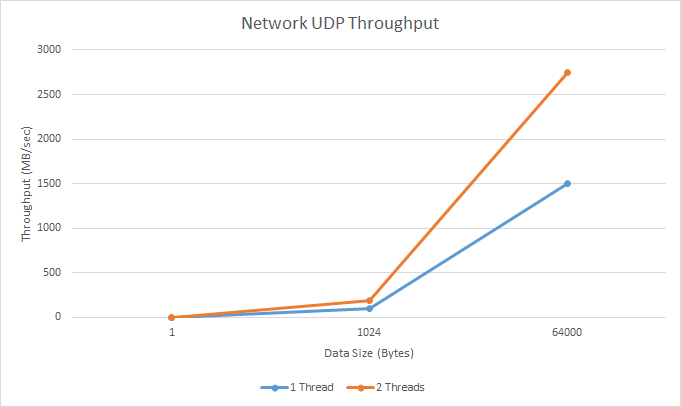
\includegraphics[width=.7\textwidth]{network_udp_throughput.png}
\caption{Network UDP Throughput Benchmark}
}
\end{figure}
\begin{figure}[H]
\center{
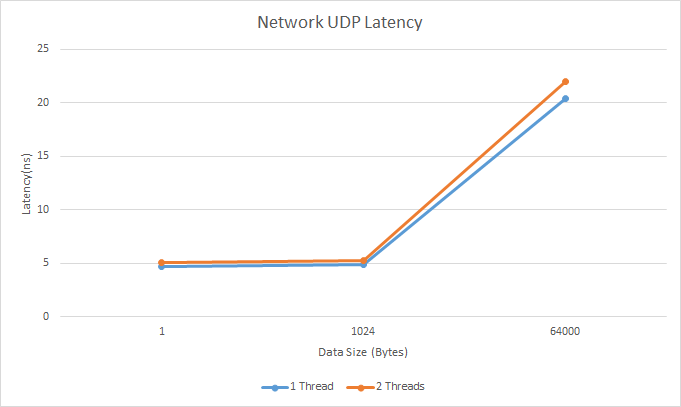
\includegraphics[width=.7\textwidth]{network_udp_latency.png}
\caption{Network UDP Latency Benchmark}
}
\end{figure}

\section{Conclusions}
Ultimately, it is difficult to simply say which settings are the "best" to use.  Different settings have different strengths and weaknesses for different projects.  Having the ability to understand and compare various metrics, as well as having an understanding of one's needs is crucial to making choices to optimize the running of a given program.

\end{document}